%####################################################################
%############ BEGIN PREAMBLE ########################################
%####################################################################
\documentclass[12pt]{report}

%Packages-------------------------------------
\usepackage{amsmath}
\usepackage{amsfonts}
\usepackage{amssymb}
\usepackage{amsthm}
\usepackage{graphics}
\usepackage{graphicx}
\usepackage{subfigure}
\usepackage{tabularx}
\usepackage[nopostdot,style=list,nonumberlist,toc]{glossaries}
%\usepackage{hyperref}
\usepackage{xurl}
\usepackage[nottoc]{tocbibind}
\usepackage{caption}
\usepackage{float}
\usepackage{setspace}

%\usepackage{xtocnic}

\usepackage[localise=on]{xepersian}

\settextfont[Scale=1]{XB Zar}
%\setdigitfont[Scale=1]{XB Zar}
\setlatintextfont[Scale=1]{Times New Roman}

%Layout---------------------------------------

%\usepackage[top=2cm, bottom=2cm, left=2cm, right=2cm]{geometry}

%Commands-------------------------------------
\setcounter{tocdepth}{3}
\setcounter{secnumdepth}{3}
\renewcommand{\arraystretch}{1.25}

%Theorems-------------------------------------
\newtheorem{thm}{قضیه}[chapter]
\newtheorem{cor}[thm]{نتیجه}
\newtheorem{defn}[thm]{تعریف}
\newtheorem{prop}[thm]{گزاره}
\newtheorem{lmm}[thm]{لم}
\newtheorem{conj}[thm]{حدس}
\newtheorem{exm}[thm]{مثال}
\newtheorem{rem}[thm]{تذکر}
\newtheorem{note}[thm]{یادداشت}
\newtheorem{alg}[thm]{الگوریتم}


%Glossaries-----------------------------------
\makeglossaries
\loadglsentries{glossaries}

%Folder of Figures----------------------------
\graphicspath{{./figures/}}
%####################################################################
%########### END PREAMBLE ###########################################
%####################################################################


%####################################################################
%########### BEGIN DOCUMENT #########################################
%####################################################################
\begin{document}
	
	%Title page ----------------------------------
	
	\begin{figure}
		\centering
		
\includegraphics[height=2.5cm]{ut.png}
	\end{figure}
	
	\begin{center}
		پردیس علوم
		\\
		دانشکده ریاضی، آمار و علوم کامپیوتر
	\end{center}
	
	\begin{center}
		%%%%%%%%%%%%%
	\end{center}
	
	\begin{center}
		\huge{مدل‌سازی سازوکارهای مسئله‌ی انقیاد در شبکه‌های عصبی ضربه‌ای}
	\end{center}
	
	\begin{center}
		%%%
	\end{center}
	
	\begin{center}
		نگارنده
	\end{center}
	\begin{center}
		\textbf{
			امیر اصلان اصلانی
			\\[30pt]
		}
	\end{center}
	
	\begin{center}
		اساتید راهنما
	\end{center}
	\begin{center}
		\textbf{
			محمد گنج‌ تابش 
			\\[5pt]
			عباس نوذری دالینی
		}
	\end{center}
	
	\vspace{3cm}
	\begin{center}
		پایان‌نامه برای دریافت درجه‌ی کارشناسی ارشد
		\\
		در رشته علوم کامپیوتر
	\end{center}
	
	\begin{center}
		بهمن ۱۴۰۱
	\end{center}
	
	\pagestyle{empty}
	\pagenumbering{}
	
	\newpage
	%\pagestyle{headings}
	%\setcounter{page}{1}
	%\pagenumbering{roman}
	\pagestyle{plain}
	\setcounter{page}{1}
	\pagenumbering{harfi}
	
	%Abstract page-------------------------------
	
	\chapter*{}
	\section*{چکیده}
	محل متن چکیده
	
	\section*{}
	\textbf{کلمات کلیدی:}\quad کلمات، کلیدی، مرتبط.
	
	%Dedication page-----------------------------
	
	%\chapter*{تقدیم به}
	%\section*{تقدیم به}
	
	%Acknowledgement page------------------------
	
	%\chapter*{سپاسگزاری}
	%\begin{center}
	%    content...
	%\end{center}
	%
	%%copyright + declaration page
	%\chapter*{اصالت اثر}
	%\section*{اصالت اثر}
	% هیچ قسمت از این پایان‌نامه، پیش از این در هیج موسسه تحصیلات عالی برای دریافت درجه تحصیلی استفاده نشده است. همچنین، هیچ قسمت از این پایان‌نامه برگردان فارسی تمامی یا قسمتی از یک اثر دیگر علمی (مانند مقاله، پایان‌نامه، و غیره) به زبانی دیگر نمی‌باشد. ارائه این پایان‌نامه توسط نگارنده به معاونت آموزشی (معاونت پژوهشی و تحصیلات تکمیلی برای ارشد و دکتری) به منزله تعهد نگارنده به اصالت متن و محتوای ارائه شده بر اساس یک کار پژوهشی در مدت تحصیل در دانشگاه تهران می باشد. در صورت اثبات خلاف این امر، مدرک تحصیلی اخذ شده توسط این پایان‌نامه از دانشگاه تهران، معتبر نمی باشد.
	%
	%\chapter*{حق مالکیت معنوی}
	%\section*{حق مالکیت معنوی}
	%حق مالکیت معنوی این اثر متعلق به دانشگاه تهران می باشد. استفاده از مطالب این پایان‌نامه در فعالیت های تحقیقاتی با ذکر منبع بلامانع می‌باشد. در صورت استفاده تجاری، مانند چاپ این پایان‌نامه، هماهنگی لازم و اجازه کتبی از دانشگاه و نگارنده پایان‌نامه الزامی می‌باشد.
	%
	
	%-------------------------
	%\pagestyle{plain}
	%\setcounter{page}{1}
	%\pagenumbering{harfi}
	%-------------------------
	\onehalfspacing
	%Preface--------------------------------------
	
	\chapter*{پیشگفتار }
	محل نگارش پیشگفتار.
	
	%Table of Contents----------------------------
	
	\tableofcontents
	%\listoffigures
	
	%#######################################################
	%#######################################################
	%#######################################################
	%#######################################################
	
	%Chapter One----------------------------------
	
	\chapter{مفاهیم اولیه}
	\label{ch:Defs}
	%*********************
	\pagestyle{plain}
	\setcounter{page}{1}
	\pagenumbering{arabic}
	%*********************
	
	در این فصل به تعریف برخی از مفاهیم اولیه خواهیم پرداخت. بدین منظور از سیستم عصبی انسان شروع و به مواردی چون ساختار اعصاب، تغیرات آن‌ها در مرور زمان، سازوکار پاداش و برخی تقسیم‌بندی‌ها درباره‌ی نواحی مغز خواهیم پرداخت و در ادامع اشاره‌ای به روش‌‌های مدلسازی رایج در موضوع شبیه‌سازی شبکه‌های عصبی خواهدشد و نهایتا با توضیحاتی در باب مسئله \gls{binding} فصل را خاتمه خواهیم داد.
	
	%=========================
	\section{سیستم عصبی انسان}
	
	به صورت کلی \gls{nervousSystem} انسان به دو بخش کلی تقسیم می‌شود؛ \gls{cns}
	\LTRfootnote{Central Nervous System (CNS)}
	و \gls{pns}
	\LTRfootnote{Peripheral Nervous System (PNS)}.
	در اینجا موضوعی که بیشتر مورد بحث می‌باشد، سیستم عصبی مرکزی، بویژه مغز می‌باشد. قشر مغز انسان به طور تخمینی از ۲۱ الی ۲۶ میلیارد نورون تشکیل شده است
	\cite{Pelvig2008-vh}
	که در بخش های بعدی با جزعیات بیشتری به ساختار و ارتباطات میان آن‌ها خواهیم پرداخت.
	
	
	اطلاعات مختلف که از ارگان‌های حسی انسان (\gls{pns}) ارسال شده‌اند در مغز تجمیع می‌شوند. سپس مغز این تصمیم را که ارگان‌های بدن چه اعمالی را باید انجام دهند، اتخاذ می‌کند. مغز داده‌های خام را برای استخراج اطلاعاتی درباره‌ی چگونگی محیط، پردازش می‌کند و سپس این اطلاعات را با نیاز‌های فعلی حیوان (میزبان) و اطلاعاتی که در حافظه از شرایط گذشته دارد ترکیب می‌کند تا نهایتا بر اساس نتایج حاصل‌شده یک الگوی حرکتی را تولید می‌کند. این پردازش اطلاعات نیازمند تعاملاتی پیچیده میان بخش‌های مختلف است 
	\cite{carew2000}.
	
	\subsection{ساختار نورون‌ها}
	
	نورون‌ها سلول‌هایی هستند که وظیفه اصلی پردازش را در سیستم عصبی موجودات بر عده دارند. به صورت خاص نورون‌ها سیگنال‌هایی را دریافت، پردازش و منتقل می‌کنند. نورون‌ها از نظر شکل، اندازه و خواص الکتروشیمیایی بسیار متنوع هستند. نورون‌ها از چند بخش اصلی تشکیل شده‌اند که به صورت زیر است:
	\begin{itemize}
		\item \gls{soma}\LTRfootnote{Soma} یا جسم سلولی که شامل هسته‌ی سلول\LTRfootnote{Nucleus} است و فعالیت‌های حیاتی سلول داخل آن اتفاق می‌افتد.
		\item \gls{dendrite}\LTRfootnote{Dendrite} که یک جسم شاخه مانند است و نقش دریافت سیگنال‌های ارسال شده توسط نورون‌های دیگر را که توسط آکسون‌های آن‌ها منتقل شده‌است را بر عهده دارد.
		\item \gls{axon}\LTRfootnote{Axon} که جسمی شاخه مانند است، سیگانال‌های ارسالی از نورون را به \gls{dendrite}‌های نورون‌های دیگر منتقل می‌کند. سرعت انتقال پیام‌‌ در این اندام متغیر است و بستگی به میزان \gls{myelin}\LTRfootnote{Myelin} اطراف آن دارد.
	\end{itemize}
	
	\begin{figure}[H]
		\centering
		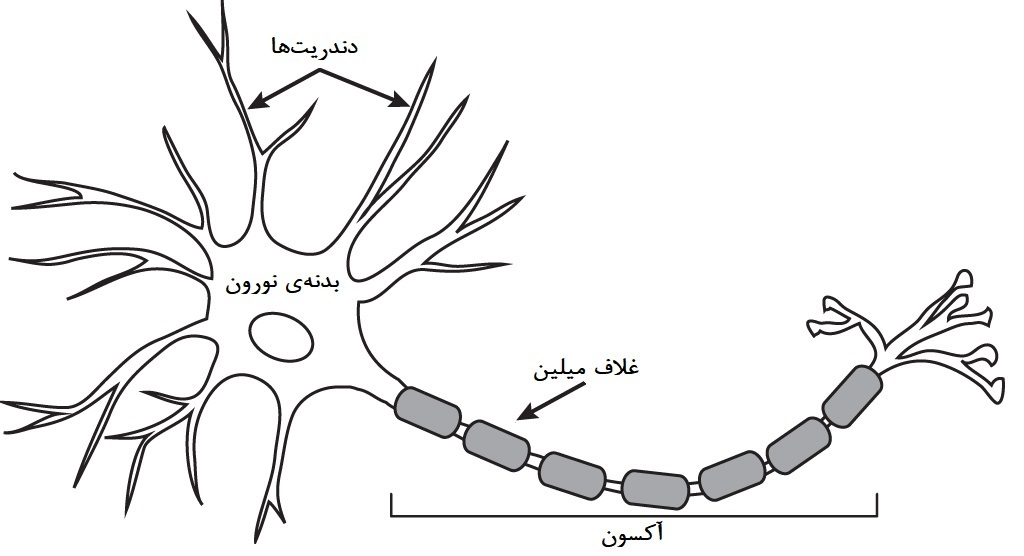
\includegraphics[width=0.7\linewidth]{neuron.jpg}
		\caption[NS]{
			اجزای تشکیل دهنده‌ی نورون\footnotemark.
		}
		\label{fig:neuron}
	\end{figure}
	
	% اینا همشون برعکس شدن (لاتین ها و اعداد. نسخه‌ی ۴ هست ولی برای درست نشون داده شدن برعکس نوشته شده)
	\RTLfootnotetext{
		خلق شده توسط
		Henley Casey 
		تحت مجوز
		BY-NC-SA CC
		نسخه ۰.۴.
	}
	
	
	نورون‌ها شامل یک لایه عایق هستند که موجب اختلاف پتانسیل مابین داخل و خارج نورون می‌شود. همچنین مجموعه‌ای از کانال‌های یونی\LTRfootnote{Ion Channels} نیز وجود دارند که نورون از طریق آنها با محیط بیرون یون‌هایی را تبادل می‌کند که این تبادلات موجب تغیر در میزان اختلاف پتانسیل نورون می‌شود. زمانی که اختلاف پتانسیل یک نورون از یک آستانه فراتر رود مجموعه‌ای از این کانال‌ها باز شده و موجب افزایش بسیار سریع اختلاف پتانسیل و سپس کاهش مجدد آن به میزان طبیعی می‌شود که به این پدیده، شلیک یا \gls{spike}\LTRfootnote{Spike} میگوییم. در زمان رخ دادن پدیده‌ی \gls{spike}، همراه با افزایش ناگهانی اختلاف پتانسیل در نورون، این اختلاف پتانسیل از طریق آکسون‌ها منتقل می‌شود و در سیناپس‌ها موجب آزاد شدن انتقال دهنده های عصبی\LTRfootnote{Neurotransmitter} می‌شود که نتیجتا باعث افزایش اختلاف پتانسیل در دندریت‌های مجاور این سیناپس‌ها می‌شود. در این پروسه به نورونی که منشا اختلاف پتانسیل انتقال داده شده بوده است را \gls{pre}‌\LTRfootnote{Pre-synaptic Neuron} و نورونی را که این اختلاف پتانسیل به آن منتقل شده است، \gls{post}‌\LTRfootnote{Post-synaptic Neuron} مینامیم.
	
	نورون‌ها از نظر عملکرد به دو دسته‌ی کلی تقسیم می‌شوند؛ دسته‌ی اول نورون‌های تحریکی\LTRfootnote{Excitatory} هستند که در سیناپس‌هایشان انتقال‌دهنده‌های عصبی تحریکی مثل گلوتامیت\LTRfootnote{Glutamate} آزاد می‌شود و باعث بیشتر شدن اختلاف پتانسیل در \gls{post} می‌شود. دسته‌ی دوم نورون‌های مهاری هستند که در سیناپس‌هایشان انتقال دهنده‌های عصبی مهاری مثل گابا\LTRfootnote{GABA} آزاد می‌شود و باعث کمتر شدن اختلاف پتانسیل در \gls{post} می‌شوند
	\cite{Purves2001-ns}.
	
	
	\subsection{انعطاف پذیری نورونی}
	
	انعطاف پذیری نورونی\LTRfootnote{Neuroplasticity} را می‌توان به عنوان توانایی سیستم عصبی برای تغیر فعالیت خودش در پاسخ به محرک درونی یا خارجی با اعمال تغیراتی در ساختار، عملکرد و اتصالات خودش قلمداد کرد
	\cite{MateosAparicio2019}.
	همچنین می‌توان پدیده‌ی یادگیری را در موجودات زنده محصول وجود انعطاف پذیری نورونی در آنها دانست.
	
	از جمله تاثیراتی که در نتیجه‌ی انعطاف پذیری نورونی ایجاد می‌شود، می‌توان به تغیر میزان تاثیر تحریکی یا مهاری \gls{pre} روی \gls{post} اشاره کرد که در نتیجه‌ی تغیر در ساختار دندیت‌ها و آکسون‌ها رخ می‌دهد.
	از جمله مهم‌ترین ‌قوانین یادگیری در این مورد، \gls{hebb}‌\LTRfootnote{H‌ebbian Learning Rule} است که به واسطه‌ی فعالیت‌های دنالد هب\LTRfootnote{Donald Hebb} معرفی شده است.
	صورت \gls{hebb} به این صورت بیان شده است: «زمانی که آکسون نورون الف به اندازه‌ای به (دندریت) نورون ب نزدیک  بود که مکررا یا دائما باعث تحریک آن شود، برخی فر‌آیند‌ها و تغیرات متابولیکی در یکی یا هر‌دوی نورو‌ن‌ها باعث تغیراتی می‌شوند تا تاثیر نورون الف در تحریک شدن نورون ب افزایش یابد»
	\cite{hebb1949organization}.
	همچنین کارلا شاتز\LTRfootnote{Carla Shatz} اینگونه قانون هب را تفسیر می‌کند: «آنهایی که همزمان ضربه میزنند، به‌هم متصل‌هم می‌شوند»
	\cite{shatz1992developing}.
	هرچند‌این تفسیر ممکن است باعث برداشت غلط شود چراکه اگر دو نورون به معنی واقعی کلمه در یک لحظه شلیک کنند امکان اینکه شلیک یکی از آن نورون‌ها معلول شلیک نورون دیگر باشد وجود نخواد داشت. بیشتر از موضوع همزمانی، موضوع ارتباط علت و معلولی بین شلیک نورون‌ها است که دارای اهمیت است
	\cite{granger1969investigating}.
	
	
	در دهه ۱۹۹۰ میلادی، آزمایش‌هایی باعث مشخص شدن پایه‌های نوروفیزیولوژی قانون هب بر اساس \gls{stdp}\LTRfootnote{Spike-timing dependent plasticity (STDP)} شدند.
	\cite{caporale2008spike} 
	مشخص شد وقتی یک نورون مهاری، به یک نورون مهاری دیگر متصل شده است، اگر \gls{pre} با فاصله‌ی زمانی ۴۰ میلی ثانیه یا کمتر نسبت به \gls{post} ضربه بزند، سیناپس‌های اتصال آن‌ها تقویت می‌شوند و اگر \gls{post} زودتر از \gls{pre} ضربه بزند، سیناپس‌های مرتبط با اتصال آن‌ها تضعیف خواهند شد. (شکل \ref{fig:stdp})
	بر اساس روابط کشف شده در تضعیف و تقویت سیناپس‌ها، می‌توان تغیرات میزان اثرگذاری نورون‌ها روی یکدیگر را به صورت زیر مدل‌سازی کرد به صورتی که $w$ میزان اثرگذاری یک نورون روی نورون دیگر، $\tau_\pm$ ثابت‌های زمانی  و $A_\pm$ میزان تغیرات وزنهای سیناپسی هستند
	\cite{gerstner2014neuronal}:
	\begin{align}
		\Delta w =
		\begin{cases}
			A_+(w).\exp(\frac{-|\Delta t|}{\tau_+})  & \text{\lr{if}}\; t_{pre} \leq t_{post}, \\
			A_-(w).\exp(\frac{-|\Delta t|}{\tau_-})  & \text{\lr{if}}\; t_{pre} > t_{post}.
		\end{cases}
		\label{eq:stdp}
	\end{align}
	
	
	\begin{figure}[H]
		\centering
		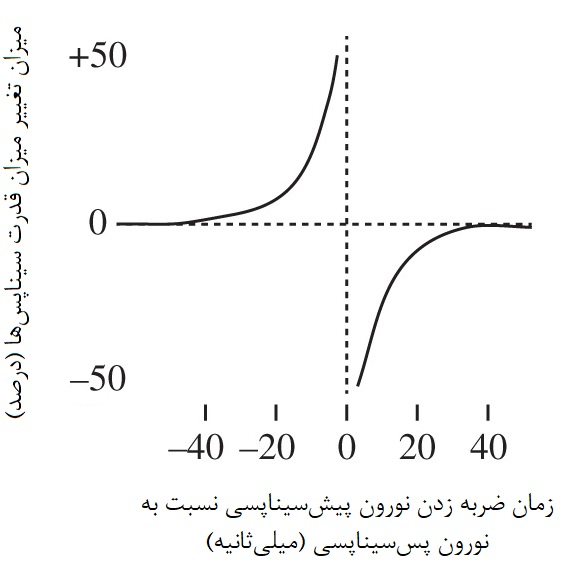
\includegraphics[width=0.7\linewidth]{stdp.jpg}
		\caption[NS]{
			میزان تقویت سیناپس ها در \gls{stdp} در فواصل زمانی مختلف.
		}
		\label{fig:stdp}
	\end{figure}
	
	
	\subsection{سازوکار پاداش در مغز}
	
	بخش بزرگی از یادگیری انسان در تعامل با محیط اتفاق می‌افتد. هر برون‌داد انسان تاثیری روی محیط پیرامونش گذاشته و محیط تغیر یافته، پس از آن تغیر، خود به عنوان یک درون‌داد از طریق سیستم عصبی محیطی درک می‌شود
	\cite{sutton1998reinforcement}.
	به توجه به درک انسان از محیط، پاداش یا تنبیه نیز برای آن در نظرگرفته می‌شود که این ساز‌و‌کار در مغز انسان بر عهده‌ی پیامرسان‌های عصبی\LTRfootnote{Neurotransmitter}  مثل دوپامین\LTRfootnote{Dopamine} است. 
	
	\begin{figure}[H]
		\centering
		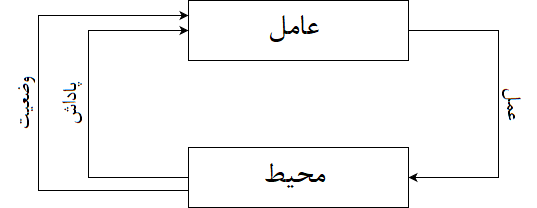
\includegraphics[width=0.7\linewidth]{rl.png}
		\caption[NS]{
			آثار عامل و محیط نسبت به یکدیگر
		}
		\label{fig:rl}
	\end{figure}
	
	تاثیر پاداش روی فعالیت اعصاب به این صورت است که برخی از نورون‌ها به این دسته از پیامرسان‌‌های عصبی حساس هستند و میزان غلظت آن‌ها روی فعالیت این دسته از نورون‌ها تاثیر گذار هستند و این تاثیر به گونه‌ای است که در صورتی که سیگنال پاداش دریافت شود، تغیرات وزن‌های اتصالات نورونی مشابه \gls{stdp} تغیر خواهند کرد؛ هرچند که میزان پاداش در شدت این تغیرات موثر است. همچنین در صورتی که سیگنال تنبیه دریافت شود تغیرات وزن‌های اتصالات بین نورونی برعکس \gls{stdp} تغیر خواهند کرد و میزان این تغیرات مشابه زمان پاداش وابسته به میزان شدت تنبیه خواهد بود.
	
	برای مدل‌سازی اثر سازوکار پاداش روی یادگیری می‌توان از روابط زیر استفاده کرد که در آنها $d$ میزان پاداش، $\delta$ تابع دیراک و $\tau_c$ به عنوان ثابت زمانی در نظر گرفته شده اند:
	
	\begin{align}
		\frac{dc}{dt} &= -\frac{c}{\tau_c} + STDP(\tau) \delta(t-t_{pre/post}) \\
		\frac{ds}{dt} &= cd
		\label{eq:rstdp}
	\end{align}
	
	
	\subsection{\gls{neocortex} و \gls{cc}}
	\gls{neocortex} یک قشر مغزی شش لایه در پستانداران است که وظیفه‌ی عملکرد‌های سطح بالایی همچون شناخت، حرکت، بینایی و زبان را برعهده دارد
	\cite{Lui2011}. نامگذاری لایه‌های \gls{neocortex} به ترتیب از بیرونی ترین لایه شماره ۱ تا درونی ترین لایه، لایه شماره ۶ می‌باشد.
	همچنین \gls{neocortex} شامل نورون های تحریکی و مهاری با نسبت تقریبی ۸۰ به ۲۰ می‌باشد
	\cite{noback2005human}.
	
	ساختار \gls{neocortex} علاوه‌بر اینکه شامل ۶ لایه افقی می‌باشد، شامل مجموعه ای از سازه‌های عمودی به نام \gls{cc} است که سطح مقطع بسیار کوچکی در ابعاد نیم میلی‌متر دارند و \gls{neocortex} از کنار‌هم قرار گرفتن این ستون‌ها شکل میگیرد
	\cite{Horton2005}.
	به صورت کلی، این ستون‌های کورتکسی از نظر ارتباط بین لایه‌ها الگوی‌های مشابه و تکرار شونده‌ای دارند که در تمام بخش های \gls{neocortex} مشابه یکدیگر هستند. مدار کورتکسی استاندارد\LTRfootnote{Canonical Cortical Circuit}، که توسط داگلاس و مارتین 
	\cite{Douglas2004}
	بیان شده، ارتباط بین بخش‌های مختلف را داخل و مابین ستون‌های کورتکسی نشان می‌دهد.
	(شکل \ref{fig:cc-doganmart})
	
	\begin{figure}[H]
		\centering
		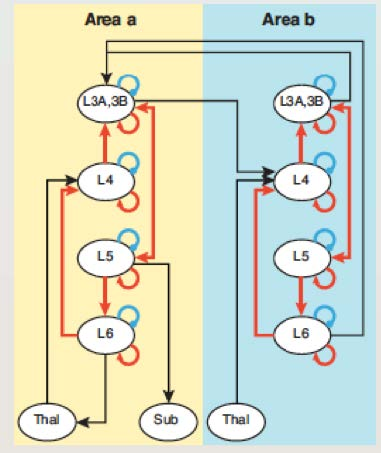
\includegraphics[width=0.5\linewidth]{cc-con.jpg}
		\caption[NS]{
			مدار کورتکسی استاندارد که توسط داگلاس و مارتین بیان شده است
			\cite{Douglas2004}.
			در این شکل پیکان‌های قرمز نشان دهنده‌ی اتصالات تحریکی و پیکان‌های آبی نشان دهنده‌ی اتصالات مهاری هستند. همانطور که در شکل نیز مشخص شده بیشتر اتصالات مهاری بین نورون‌های یک لایه‌ی مشخص هستند. همچنین پیکان‌های مشخص شده با رنگ مشکی نشانگر اتصالات بین دو ستون کورتکسی مجزا هستند.
		}
		\label{fig:cc-doganmart}
	\end{figure}
	
	
	\section{مسئله‌ی \gls{binding}}
	
	در حوزه‌های علوم اعصاب، علوم شناختی و فلسفه ذهن مسئله‌ای تحت عنوان مسئله‌ی \gls{binding}
	\LTRfootnote{Binding Problem}
	یا ترکیب 
	\LTRfootnote{Combination Problem}
	مطرح می‌شود که در ادامه به پاره‌ای از موضوعات حول آن خواهیم پرداخت.
	
	\subsection{صورت مسئله‌ی \gls{binding}}
	مسئله‌ی \gls{binding} به چگونگی پردازش مفاهیم مجزا همچون اشیاء و ویژگی‌های انتزاعی و احساسی به صورت یک مفهوم گسترده‌تر تجمیع شده میپردازد
	\cite{REVONSUO1999123}.
	
	به صورت عمومی این مسئله به چگونگی در‌هم آمیختن مفاهیم مختلف درک شده و تجمیع آن‌ها به صورت یک تجربه‌ی واحد میپردازد
	\cite{Feldman2012}.
	همچنین دلیل اینکه از \gls{binding} به عنوان یک مسئله یاد می‌شود این است که هنوز به صورت کامل از سازوکار آن اطلاعی در دست نیست.
	
	\begin{figure}[H]
		\centering
		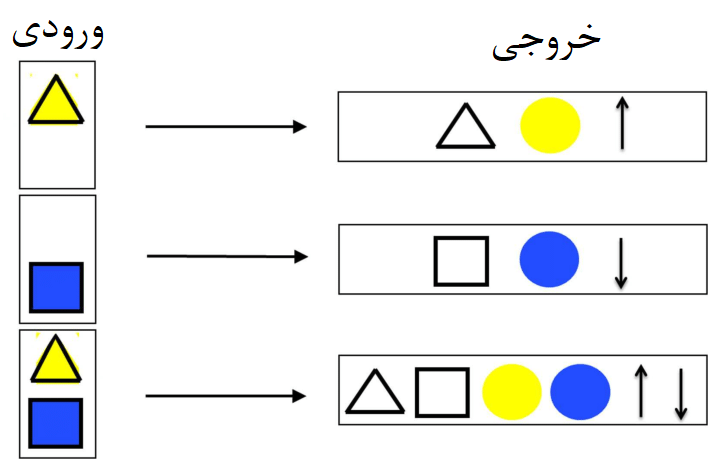
\includegraphics[width=0.7\linewidth]{binding.png}
		\caption[NS]{
			یک نمایش از تعریف کلاسیک \gls{binding} و چگونگی ادراک مفاهیم جامع توسط درک مفاهیم جزئی‌تر
			\cite{velic2012}.
		}
		\label{fig:binding}
	\end{figure}
	
	
	\subsection{شواهد رخ‌دادن \gls{binding} در انسان}
	
	آنه تریسمن\LTRfootnote{Anne Treisman}
	و هیلاری اشمیت\LTRfootnote{Hilary Schmidt}
	آزمایشی را انجام دادند که در آن به مطالعه اثری با نام ترکیب‌های توهمی\LTRfootnote{Illusory Conjunctions}
	پرداختند که در آن آزمایش ویژگی‌های یک شئ به شئ دیگری منتسب می‌شود
	\cite{TREISMAN1982107}.
	بر اساس نظر تریسمن، علت این انتصاب اشتباه در ویژگی‌های اشیاء، حضور جدا از هم صفات در مراحل اولیه ادراکی است
	\cite{goldstein_2019}.
	اهمیت این موضوع از این جهت است که حالت ممکن دیگر آن است که یک شئ نه به صورت صفات جداگانه، بلکه به صورت یک ماهیت کامل حاضر شود. این در حالی است که رخ دادن مسئله‌ی \gls{binding} در مغز مستلزم حضور ویژگی‌ها و صفات به صورت جدا از هم می‌باشد که این آزمایش نشانگر اتفاق افتادن \gls{binding} در مغز است.
	
	
	\section{\gls{snn}}
	شبکه‌های عصبی مصنوعی\LTRfootnote{Artificial Neural Networks} بر پایه دینامیک‌های بسیار ساده شده مغز ساخته شده‌اند و به عنوان یک ابزار محاسباتی قوی برای حل بسیاری از مسائل استفاده می‌شوند
	\cite{TGNN}. 
	\gls{snn}\LTRfootnote{Spiking Neural Networks} نوعی از شبکه‌های عصبی مصنوعی هستند که در آن ارتباط بین نورون‌ها توسط ضربه‌ها و سیناپس‌ها  با وزن‌های متغیر، مطابق با مشاهدات زیستی تعریف شده‌اند
	\cite{ghosh2009spiking}. 
	از جمله مهمترین ویژگی هایی که در \gls{snn} در نظر گرفته شده، بعد زمان است
	\cite{Mozafari2019}
	که این مورد در شبکه‌های عصبی کلاسیک در نظر گرفته نمی‌شده. در \gls{snn} اطلاعات میتوانند در زمان‌های مختلفی منتقل شوند و زمان خود در مفهوم منتقل شده نقش مهمی را بازی میکند
	\cite{SNN1997}.
	
	برای شبیه‌سازی این گونه از شبکه‌های عصبی، سازوکار نورون‌های زیستی به روش‌‌های گوناگونی مدل‌سازی شده‌اند که ازجمله ساده ترین‌ها که در عین‌حال کارایی بسیار مناسبی را دارد مدل نورونی \gls{lif}\LTRfootnote{Leaky integrate-and-fire} است که در ادامه به آن خواهیم پرداخت.
	
	
	\subsection{مدل نورونی \gls{lif}}
	در مدل نورونی \gls{lif} تلاش شده تا ویژگی‌ها و خواص مهم نورون‌های بیولوژیکی لحاظ شوند. در این نورون‌ها با وارد شدن ضربه‌های تولید شده توسط نورون‌های پیش‌سیناپسی به نورون، اختلاف پتانسیل آن افزایش می‌یابد (تجمیع) و در صورت رسیدن اختلاف پتانسیل به یک آستانه‌ی مشخص، این نورون خود ضربه‌ای تولید میکند (آتش) که توسط اتصالات بین نورونی به نورون‌های پس‌سیناپسی منتقل میشوند. همچنین در گذر زمان اختلاف پتانسیل نورون به مرور در حال کاهش به سمت یک میزان مشخص اختلاف پتانسیل است (نشتی) که به آن اختلاف پتانسیل استراحت می‌گوییم
	\cite{gerstner2014neuronal}.
	
	ساز‌وکار بیان شده برای تغیرات اختلاف پتانسیل را در این مدل نورونی میتوان به صورت معادلات دیفرانسیل بیان شده در رابطه‌ی \ref{eq:lif} بیان کرد که در آن $u$ اخلاف پتانسیل فعلی نورون، $u_{rest}$ اختلاف پتانسیل استراحت، $I(t)$ جریان ورودی به نورون و $R$ مقاومت الکتریکی قشای نورون را نشان می‌دهند
	\cite{gerstner2014neuronal}.
	
	\begin{align}
		\tau . \frac{du}{dt} = -(u - u_{rest}) + R . I(t) 
		\label{eq:lif}
	\end{align}
	
	
	\chapter{طرح مسئله}
	
	در این فصل به اهمیت مدل‌سازی مسئله‌ی \gls{binding} و مسائلی که درک بیشتر ما از این موضوع آن‌ها را نیز تحت تاثیر قرار خواهد داد، خواهیم پرداخت که از‌جمله آن‌ها میتوان به هوش مصنوعی و درک بهتر ساز‌وکار مغز اشاره کرد.
	
	\section{مشکلات موجود حاضر}
	
	با توجه به چالش‌های حال حاضر، درک چگونگی اتفاق افتادن \gls{binding} در مغز، از اهمیت بالایی برخوردار است؛ زیرا با توجه به اهمیت و میزان تاثیر \gls{binding} در آگاهی و درک موجود زنده از محیط خود، به این موضوع در مسائلی همچون درک و شبیه‌سازی هوش انسانی که یکی از چالش‌های هوش مصنوعی است، نیاز است.
	
	در راستای دست‌یابی به سیستم‌های هوشمند فعالیت‌های بسیاری انجام شده است که از جمله‌ موفق ترین و موثر ترین روش‌های حاضر، استفاده از شبکه‌های عصبی مصنوعی است که یک روش الهام گرفته شده از سیستم عصبی انسان است و در حال حاضر به صورت گسترده مورد استفاده قرار گرفته‌اند. این روش در  عین این‌که در شرایط مناسب از بهره‌وری بسیار خوبی برخوردار است و امکان دست‌یابی به نتایج بسیار خوبی را در مدل‌سازی آماری داده‌های جهان دارد، به میزان داده‌ی بسیار زیادی برای آموزش نیاز دارد، در انتقال مفاهیم از پیش آموخته شده به مسائل جدید نیز با مشکل مواجه است و امکان تعمیم و عمومی سازی مسائل آموخته‌شده را ندارند.
	از جمله اصلی ترین دلایل مشکلات و محدودیت‌های موجود در شبکه‌های عصبی مصنوعی، ناتوانی آن‌ها در شکل‌دهی، بازنمایی و ارتباط بین مفاهیم و موجودیت‌ها است. به خوبی نشان داده شده است که درک انسان حول اشیاء شکل گرفته است که این اشیاء میتوانند به صورت مستقل پردازش شوند و به حالت‌های بسیار زیادی دوباره با یکدیگر ترکیب شوند و این مسئله به انسان امکان تعمیم درک خود به مسائل فراتر از تجربیاتش را می‌دهد که این ساز‌وکار همان رویه مورد بررسی در مسئله‌ی \gls{binding} است
	\cite{greff2020binding}.
	
	\section{عملکرد شبکه‌های عصبی ضربه‌ای در مسائل مطرح شده}
	شبکه‌های عصبی ضربه‌ای در مقایسه با شبکه‌های عصبی کلاسیک از توجیه زیستی بسیار بیشتری برخوردار هستند و در آن‌ها جزعیات نورون‌های زیستی بسیار بیشتر در نظر گرفته شده است که این موضوع پتانسیل‌های این دسته از شبکه‌هارا نیز تحت تاثیر قرار میدهد. در این دسته از شبکه‌ها به دلیل انتقال داده‌ها با در نظر گرفتن زمان و در قالب ضربه (بجای عدد در شبکه‌‌های عصبی کلاسیک) امکان درک مفاهیم به صورت اشیاء بجای مدل‌سازی آماری در آن‌ها بسیار محتمل‌تر است و به همین دلیل این امکان وجود دارد که بتوان در این دسته از شبکه‌های عصبی سازوکاری را تحت شرایط مشخصی به‌وجود آورد که در آن مسائل و مشکلات مطرح شده دیگر رخ ندهند و به عبارتی در این دسته از شبکه‌های عصبی میتوان انتظار اتفاق افتادن \gls{binding} را داشت.
	
	\section{تعریف مسئله}
	همواره شبیه‌سازی و درک ساختار‌های موجود در مغز انسان جزو مسائل مورد اهمیت برای انسان‌ها بوده است و در دهه‌های اخیر نیز با رشد و گسترش قدرت محاسباتی و علومی چون هوش مصنوعی و علوم اعصاب این اهداف بسیار در دسترس تر از پیش به نظر میرسند و فعالیت‌های بسیاری نیز در دهه های اخیر در رابطه با این موضوع آغاز شده است که از جمله‌ی آن‌ها میتوان به پروژه مغز آبی\LTRfootnote{Blue Brain Project} و پروژه‌ی مغز انسان\LTRfootnote{Human Brain Project (HBP)} اشاره کرد.
	
	چنانچه پیشتر مطرح شد، مسئله‌ی \gls{binding} به عنوان یکی از مهمترین مسائل در شناخت مغز و هوش مصنوعی، که تقریبا در تمام فعالیت‌های شناختی پستانداران در حال رخ دادن است، برای شبیه‌سازی در شبکه‌های عصبی مصنوعی کلاسیک که صرفا نرخ ضربه با کد میکنند\LTRfootnote{Rate-coding} با محدودیت‌هایی مواجه است \cite{vonderMalsburg1999} که این موضوع را در دسته‌ی مسائل حل نشده قرار داده است. ولی در سال‌های اخیر با افزایش قدرت پردازشی و پیشرفت شبکه‌های عصبی ضربه‌ای‌، امید است تا بتوان با استفاده از این نسل از شبکه‌های عصبی مصنوعی مسیر جدیدی در درک و شبیه‌سازی مسئله‌ی \gls{binding} را در پیش گرفت که به نتایج بهتری نسبت به انواع کلاسیک در آن رسید.
	
	همچنین استفاده شبکه‌های عصبی ضربه‌ای این امکان را برای ما فراهم میکند که در ساختار و توپولوژی شبکه نیز از ساختار‌های طبیعی مغز بیش از پیش الگوبرداری کرد. این موضوع از این جهت  حائز اهمیت است که \gls{binding} در مغز پستانداران در حال رخ دادن است و هرچه بیشتر مکانیز ها و شبکه‌ی شبیه‌سازی شده، بیشتر شبیه نمونه‌ی طبیعی خود باشند احتمال رخ دادن \gls{binding} نیز در شبیه‌سازی بیشتر خواهد بود.
	
	در مطالعه‌ی پیش‌رو در تلاش خواهیم بود تا با استفاده از شبکه‌های عصبی ضربه‌ای و الگو برداری از ساختار و توپولوژی مغز پستانداران یک شبکه‌ی عصبی را شبیه‌سازی کنیم و در آن وجود آثاری از رخ دادن \gls{binding} را بررسی کنیم.
	
	
	\chapter{تحقیقات پیشین}
	
	در این فصل مجموعه‌ای از تحقیقات انجام شده پیرامون مسئله‌ی \gls{binding} و نظریه‌هایی پیرامون چگونگی رخ داد آن در مغز و \gls{snn} را بررسی خواهیم کرد.
	
	
	\section{پیدایش \gls{binding} در گروه‌های چندزمانی}
	اگوچی و همکارانش در پژوهشی
	\cite{EGUCHI2018a}
	با ساخت یک شبکه‌ی عصبی سلسله مراتبی که لحاظ کردن تاخیر انتقال آکسونی\LTRfootnote{Axonal Transmission Delay} در آن باعث شده تا در زیرجمعیت‌های آن گروه‌های چندزمانی\LTRfootnote{Polychronization}\cite{Izhikevich2006-dy} شکل بگیرند که هریک از آن‌ها به یک الگوی تصادفی با توزیع پواسون حساس شده بودند، نشان دادند که \gls{binding} بین مفاهیم دیداری سطح پایین و سطح بالا به مرور زمان شکل میگیرد که در این شبکه هریک از این مفاهیم در قالب فعالیت یک گروه چندزمانی در نظر گرفته شده بودند.
	
	مثالی از نمود بسیار ساده‌ی \gls{binding} در این شبکه در شکل \ref{fig:eguchi-binding} نشان داده شده است که در آن به دلیل وجود تاخیر در انتقال، وقتی چند مفهوم که هریک به یک یا مجموعه‌ای از نورون‌ها مقید شده اند، در فواصل زمانی مشخصی به شبکه داده شوند باعث فعال شدن یک مفهوم سطح بالاتر که شامل مفاهیم سطح پایین‌تر نیز میباشد، میشوند. 
	
	\begin{figure}[H]
		\centering
		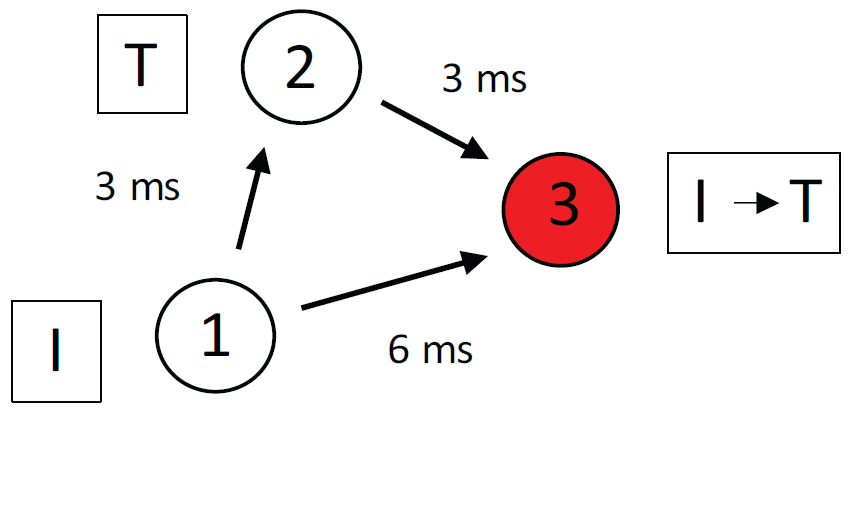
\includegraphics[width=0.7\linewidth]{poly-bind.png}
		\caption[NS]{
			یک مثال فرضی از انقیاد در سطح نورونی که در آن نورون شماره ۱، یک ویژگی سطح پایین مثل یک خط عمودی را نمایندگی میکند و نورون شماره ۲ نیز یک ویژگی سطح بالاتر مثل تصویر حرف T را نمایندگی میکند و نورون شماره ۳ انقیاد را مشخص میکند. به عبارتی نورون ۳ فعال میشود اگر و تنها اگر نورون ۱ در فعال شدن نورون ۲ نقش مستقیم داشته باشد.
		}
		\label{fig:eguchi-binding}
	\end{figure}
	
	پدیده‌ی مطرح شده میتواند بین گروه‌های چندزمانی نیز رخ دهد. به عبارتی \gls{binding} میتواند بین گروه‌های چندزمانی که نماینده‌ی یک مفهوم مستقل هستند رخ دهد و با یک گروه چند زمانی دیگر نمایندگی شود که نمونه‌ی آن نیز در شکل \ref{fig:eguchi-binding-group} قابل مشاهده است.
	
	\begin{figure}[H]
		\centering
		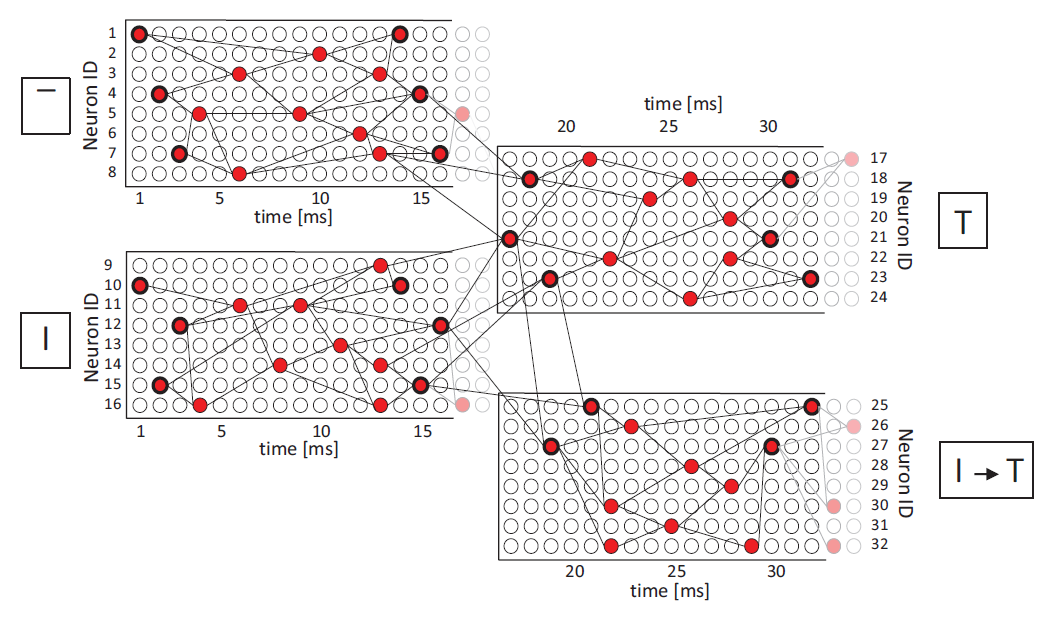
\includegraphics[width=0.7\linewidth]{poly-group-bind.png}
		\caption[NS]{
			نمود رخ دادن مثال ذکر شده در شکل \ref{fig:eguchi-binding}  از \gls{binding} در گروه های چند زمانی.
		}
		\label{fig:eguchi-binding-group}
	\end{figure}
	
	\section{ستون‌های کورتکسی، واحد‌های مستقل محاسباتی}
	هاوکینز در کتابی \cite{Hawkins2021-rq} که حاصل از مجموعه تحقیقات هاوکینز و همکارانش
	\cite{Hawkins2016, Hawkins2017, Lewis2019}
	بود، با فرض اینکه ستون‌های کورتکسی در سراسر نئوکورتکس ساختار‌های مشابهی دارند و عملکرد آن‌ها صرفا به دلیل تفاوت ورودی‌های آن‌ها است \cite{Mountcastle1978} یک مدل نورونی برای حل مسئله‌ی \gls{binding} پیشنهاد داد. با فرض اینکه هر ستون کورتکسی مسئولیت درک مفهومی را بر عهده دارد و با علم بر این که میتواند بین لایه‌های متناظر برخی ستون‌های کورتکسی با فاصله‌ی مکانی بالا، اتصالات از راه دور\LTRfootnote{Long-distance connections} شکل بگیرد، این فرضیه را مطرح کرد که این اتصالات از راه دور می‌توانند به وجود آورنده‌ی نوعی مکانیزم رای‌گیری باشند که نهایتا موجب شکل گیری \gls{binding} در مغز میشوند.
	
	برای انجام شدن رای گیری، هر ستون کورتکسی با توجه به داده‌های ورودی خود، در صورت حضور مجموعه‌ای از مفاهیم فعال خواهد بود و برای دیگر مفاهیم فعالیت کمتری خواهد داشت. با استفاده از اتصالات از راه دور هر ستون کورتکسی فعالیت و عدم فعالیت خود را به دیگر ستون‌های کورتکسی مخابره میکند و در ستون‌های کورتکسی دیگر، مفاهیم محتمل‌تر، مفاهیم با احتمال پایین‌تر را خنثی کرده و نهایتا از روی فعالیت چندین ستون کورتکسی یک مفهوم جامع‌تر حاصل شده از فعالیت دیگر ستون‌ها شکل میگیرد.
	
	مدل پیشنهادی آن‌ها (شکل \ref{fig:hawkins2017}) برای ستون‌های کورتکسی، یک مدل دو لایه‌ است که ورودی ستون کورتکسی وارد یکی از لایه‌ها شده و از آن لایه پس از پردازش به لایه‌ی دیگر منتقل میشود و سپس از لایه‌‌ی دوم از طریق اتصالات از راه دور به لا‌‌یه‌های دوم دیگر ستون‌های کورتکسی منتقل میشوند. همچنین آن‌ها مجموعه‌ای از اتصالات بازخورد\LTRfootnote{F‌‌‌eedback Connections} را نیز از لایه‌ی دوم به لا‌یه‌ی اول تعریف کردند که وظیفه‌ی آن‌ها ارائه‌ی یک پیش‌نمایش از مفهوم‌ شکل گرفته در لايه‌ی دوم است که باعث تعادل و هماهنگی بین دو لایه‌ می‌شود. در مطالعه‌ی صورت گرفته توسط ایشان\cite{Hawkins2017} مفهوم مورد بررسی، درک موقعیت‌های مکانی از روی داده‌های مربوط به حس لامسه بوده است و انتظار آن‌ها شکل گرفتن یک فعالیت با ثبات متناظر با مکان مورد لمس، در لایه‌ی دوم بدون لحاظ شدن حالت خود شئ (زاویه و جهت) بوده. 
	
	\begin{figure}[H]
		\centering
		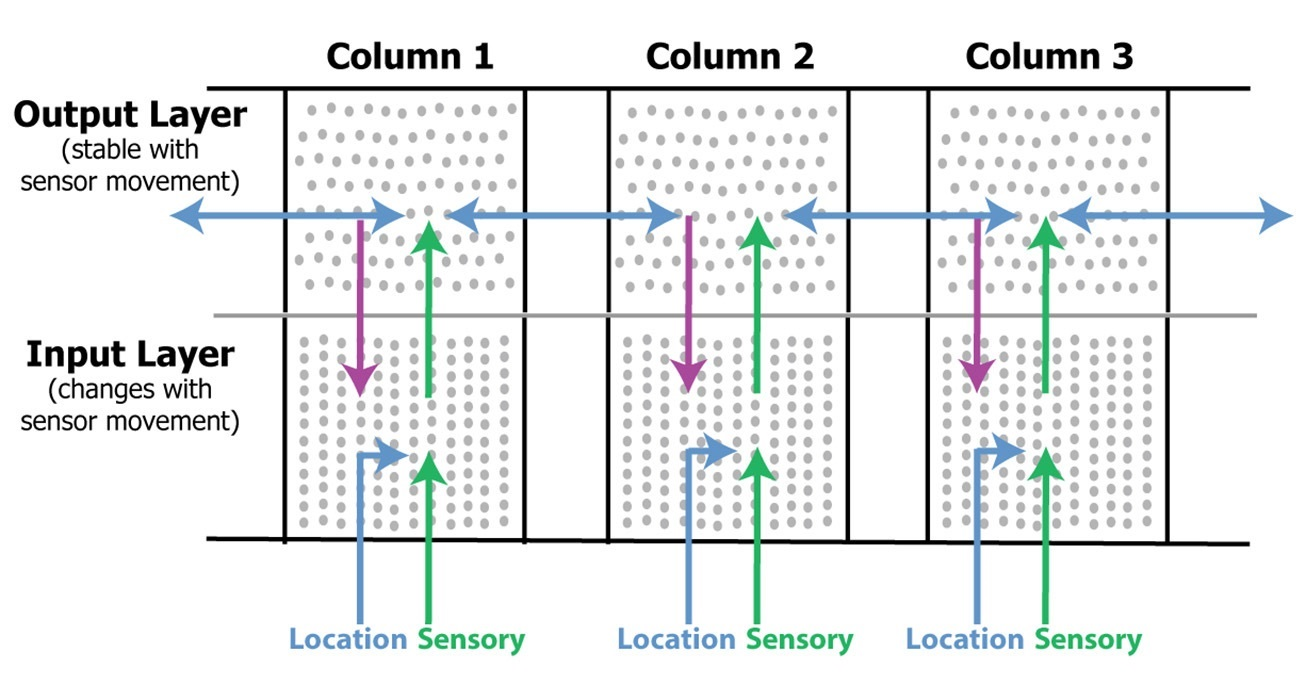
\includegraphics[width=1.0\linewidth]{hawkins2017.jpg}
		\caption[NS]{
			مدل پیشنهادی در مطالعه‌ی صورت گرفته \cite{Hawkins2017} برای درک موقعیت‌های مکانی با استفاده از داده‌های مربوط به لامسه و حرکت انگشت‌ها.
		}
		\label{fig:hawkins2017}
	\end{figure}
	
	\chapter{مدل پیشنهادی، آزمایش‌ها و نتایج}
	
	
	\chapter{جمع‌بندی و پیشنهاد کار‌های آینده}
	
	
	%#######################################################
	%#######################################################
	%#######################################################
	%#######################################################
	
	
	
	%Glossaries-----------------------------------
	
	\printglossary[title=واژه‌نامه فارسی به انگلیسی, toctitle=واژه‌نامه فارسی به انگلیسی]
	
	%References-----------------------------------
	
	%\begin{thebibliography}{MM}
	\begin{latin}
		\bibliographystyle{abbrv}
		\renewcommand{\bibname}{\rl{{مراجع}\hfill}}
		%	\addcontentsline{toc}{chapter}{کتاب‌نامه}
		\bibliography{references}
	\end{latin}
	%\end{thebibliography}
	
	%Abstract En----------------------------------
	\linespread{1}
	\begin{latin}
		\begin{abstract}
			place holder
			
			\section*{}
			\textbf{Keywords:}\quad relative, key, words.
		\end{abstract}
		\newpage
		
		%Title page En -------------------------------
		\begin{figure}
			\centering
			
\includegraphics[height=2.5cm]{ut.png}
		\end{figure}
		\begin{center}
			
			College of Science\\
			School of Mathematics, Statistics, and Computer Science
		\end{center}
		
		\begin{center}
			%%%%%%%%%%%%%
		\end{center}
		
		\begin{center}
			\huge{Modeling the Mechanisms of Binding Problem in Spiking Neural Networks}
		\end{center}
		
		\begin{center}
			%%%
		\end{center}
		
		\begin{center}
			\textbf{
				Amir Aslan Aslani
				\\[30pt]
			}
		\end{center}
		
		
		\begin{center}
			Supervisors
		\end{center}
		\begin{center}
			\textbf{
				Mohammad Ganjtabesh
				\\[5pt]
				Abbas Nouzari Dalini
			}
		\end{center}
		
		
		\vspace{3cm}
		\begin{center}
			A thesis submitted to Graduate Studies Office\\
			in partial fulfillment of the requirements for the degree of \\
			Master of Science in\\
			Computer Science
		\end{center}
		
		\begin{center}
			February 2022
		\end{center}
		
		%\pagestyle{empty}
		%\pagenumbering{}
		
	\end{latin}
	
\end{document}
%####################################################################
%########### END DOCUMENT ###########################################
%####################################################################